\documentclass[12pt]{article}

%%======== PACKAGES & PAGE SETUP ========
\usepackage[utf8]{inputenc}
\usepackage[T1]{fontenc}
\usepackage{newtxtext}
\usepackage{amsmath,amssymb,amsfonts,amsthm}
\usepackage{mathtools}
\usepackage{bm}
\usepackage{enumitem}
\usepackage[a4paper, hmargin=2.5cm, vmargin=3cm]{geometry}
\usepackage{setspace}
  \setstretch{1.35}
\usepackage{graphicx,booktabs,float}
\usepackage{xcolor}
  \definecolor{buRed}{HTML}{CC0000}
\usepackage{tikz}
  \usetikzlibrary{calc}
\usepackage{hyperref}
  \hypersetup{colorlinks=true, linkcolor=blue, urlcolor=blue, citecolor=blue, pdfborder={0 0 0}}
\usepackage{listings}
\lstdefinestyle{pseudo}{basicstyle=\ttfamily\footnotesize, columns=fullflexible,
  keepspaces=true, breaklines=true, frame=single, framesep=5pt,
  rulecolor=\color{gray!50}, showstringspaces=false}
\lstdefinestyle{code}{language=Python, basicstyle=\ttfamily\scriptsize,
  keywordstyle=\color{blue!70!black}, commentstyle=\color{gray}, stringstyle=\color{buRed!80!black},
  showstringspaces=false, breaklines=true, numbers=left, numberstyle=\tiny\color{gray},
  frame=single, rulecolor=\color{gray!50}}
\usepackage{fancyhdr}
  \pagestyle{fancy}
  \fancyhf{}
  \fancyfoot[C]{\thepage}
  \renewcommand{\headrulewidth}{0pt}

%%======== HOMEWORK MACROS ========
\newcommand{\hwNumber}{\#13}
\newcommand{\hw}{Homework}
\newcommand{\E}{\mathbb{E}}
\newcommand{\PP}{\mathbb{P}}
\newcommand{\VaR}{\mathrm{VaR}}
\newcommand{\1}{\mathbf{1}}
\theoremstyle{remark}
\newtheorem*{remark}{Remark}

%%======== BU LOGO ========
\newcommand{\buLogo}[2][]{%
  \begin{tikzpicture}[#1]
    \pgfmathsetlengthmacro{\BUwidth}{#2}
    \pgfmathsetlengthmacro{\BUheight}{#2 * 1.5 / 5}
    \fill[buRed] (0,0) rectangle (\BUwidth,\BUheight);
    \draw[white, line width=1.5pt] (0,0) rectangle (\BUwidth,\BUheight);
    \draw[white, line width=0.8pt]
      ($(0,0)+(2pt,2pt)$) rectangle ($(\BUwidth,\BUheight)+(-2pt,-2pt)$);
    \node[text=white, anchor=center, font=\fontsize{30pt}{44pt}\selectfont]
      at (0.5*\BUwidth, 0.70*\BUheight) {BOSTON};
    \node[text=white, anchor=center, font=\normalfont\fontsize{20pt}{28pt}\selectfont,
      text width=\BUwidth, align=center]
      at (0.5*\BUwidth, 0.30*\BUheight) {UNIVERSITY};
  \end{tikzpicture}%
}

\newcommand{\GridDist}{0.0008}
\newcommand{\GridLo}{12.49}
\newcommand{\GridHi}{17.51}
\newcommand{\AvgArc}{15.55}
\newcommand{\RangeOverAvg}{32}

\newcommand{\su}{\sigma_1^u}
\newcommand{\sd}{\sigma_1^d}

%%======== DOCUMENT ========
\begin{document}

\begin{titlepage}
\begin{center}
  \vspace*{2cm}
  \buLogo{7cm}

  \vspace{1em}
  \textbf{Questrom School of Business\\}
  \vfill
  \textbf{MF731: Corporate Risk Management \\}
  \textbf{Qingshuo Song \\}
  {\hw\ \hwNumber: Many Models, One Market: Calibration and Model Risk \\}
  \vfill
  \textbf{Nabizhan Bobokhanov \\}
  (Student ID: U19132437) \\
  \vfill
  \fbox{\parbox{0.8\textwidth}{\centering\small \textbf{Code:} \url{https://github.com/nabizhka/calibration-hw}\\ (the full source is also listed in the Appendix)}}
\end{center}
\end{titlepage}

\section*{Setup}
With $r=0$ the tree moves $S_{n+1}=S_n(1+\sigma_nZ_{n+1})$, $Z=\pm1$. The discounted price is a
$\mathbb Q$-martingale iff $\E^{\mathbb Q}[Z]=0$, so each branch has risk-neutral probability $\tfrac12$
and each of the four leaves at time 2 has probability $\tfrac14$. The quoted options are at the money,
strike $S_0$:
\[
C^m(1,S_0)=\E^{\mathbb Q}[(S_1-S_0)^+]=\frac{\lambda_1S_0}4,\qquad
C^m(2,S_0)=\E^{\mathbb Q}[(S_2-S_0)^+]=\frac{\lambda_2S_0}4 .
\]
\textbf{Reading.} The volatilities are taken in $[0,1]$: $\sigma\ge0$ fixes which branch is ``up'', and
$\sigma\le1$ keeps prices non-negative. (Negative $\sigma$ only relabels the branches.) Where an
endpoint $\sigma=0$ matters, I say so.

%-------------------------------------------------------------------------------
\section*{1. $\sigma_0=\lambda_1/2$}
At time 1, $S_1^u-S_0=S_0\sigma_0\ge0$ and $S_1^d-S_0=-S_0\sigma_0\le0$, so
\[
C^Q(1,S_0)=\tfrac12\,S_0\sigma_0+\tfrac12\cdot0=\tfrac{S_0\sigma_0}2 .
\]
Setting this equal to $\lambda_1S_0/4$ gives $\sigma_0=\lambda_1/2$. \qed

%-------------------------------------------------------------------------------
\section*{2. The equation for $(\su,\sd)$}
With $\sigma_0=\lambda_1/2$ we have $1+\sigma_0=s_+$ and $1-\sigma_0=s_-$, where $s_\pm=1\pm\lambda_1/2$.
The four excesses over the strike are
\begin{align*}
S_2^{uu}-S_0&=S_0\bigl[s_+(1+\su)-1\bigr]=S_0\bigl[\tfrac{\lambda_1}2+\su s_+\bigr]\ \ge0,\\
S_2^{ud}-S_0&=S_0\bigl[s_+(1-\su)-1\bigr]=S_0\bigl[\tfrac{\lambda_1}2-\su s_+\bigr],\\
S_2^{du}-S_0&=S_0\bigl[s_-(1+\sd)-1\bigr]=S_0\bigl[-\tfrac{\lambda_1}2+\sd s_-\bigr],\\
S_2^{dd}-S_0&=S_0\bigl[s_-(1-\sd)-1\bigr]=S_0\bigl[-\tfrac{\lambda_1}2-\sd s_-\bigr]\ \le0,
\end{align*}
using $s_+-1=\lambda_1/2$ and $s_--1=-\lambda_1/2$. The first is always in the money, so its
positive part is itself; the last never is, so it contributes $0$. Hence
\[
\frac{\lambda_2S_0}4=C^Q(2,S_0)=\frac{S_0}4\Bigl[\tfrac{\lambda_1}2+\su s_++\bigl(\tfrac{\lambda_1}2-\su s_+\bigr)^++\bigl(-\tfrac{\lambda_1}2+\sd s_-\bigr)^+\Bigr],
\]
and dividing by $S_0/4$ gives the stated equality. \qed

\textbf{A shorter form.} For $c,x$ real, $c+x+(c-x)^+=c+\max(c,x)$. With $c=\lambda_1/2$:
\[
\lambda_2=\frac{\lambda_1}2+\max\Bigl(\frac{\lambda_1}2,\ \su s_+\Bigr)+\Bigl(\sd s_--\frac{\lambda_1}2\Bigr)^+.\tag{$\ast$}
\]

%-------------------------------------------------------------------------------
\section*{3. $\lambda_1<2\max\{\su s_+,\sd s_-\}$}
Suppose not: $\su s_+\le\lambda_1/2$ and $\sd s_-\le\lambda_1/2$. Then in $(\ast)$ the max equals
$\lambda_1/2$ and the positive part is $0$, so $\lambda_2=\lambda_1$. This contradicts the assumption
$\lambda_1<\lambda_2$. So at least one of $\su s_+,\sd s_-$ exceeds $\lambda_1/2$. \qed

\textbf{What it says.} If both second-period volatilities are small enough that the middle leaves stay
on their own side of the strike, the time-2 call is worth exactly the time-1 call. Time value
beyond period 1 requires one of the middle leaves to cross the strike.

%-------------------------------------------------------------------------------
\section*{4. The solution set for $\lambda_1=.2$, $\lambda_2=.4$}
Now $\lambda_1/2=.1$, $s_+=1.1$, $s_-=.9$, and $(\ast)$ reads
\[
\max(.1,\ 1.1\su)+(.9\sd-.1)^+=.3 .
\]
The kinks are at $\su=.1/1.1=1/11$ and $\sd=.1/.9=1/9$. Four cases:
\begin{enumerate}[leftmargin=*]
\item $\su\le1/11$, $\sd\le1/9$: the left side is $.1\ne.3$. No solutions (this is Question 3).
\item $\su\le1/11$, $\sd>1/9$: $.1+.9\sd-.1=.3$, so $\sd=1/3$.
\item $\su>1/11$, $\sd\le1/9$: $1.1\su=.3$, so $\su=3/11$.
\item $\su>1/11$, $\sd>1/9$: $1.1\su+.9\sd-.1=.3$, i.e.\ $1.1\su+.9\sd=.4$. Within the case, $\su$
runs from $1/11$ (where $\sd=1/3$) to $3/11$ (where $\sd=1/9$).
\end{enumerate}
All values are in $[0,1]$, and the pieces join, so the calibrated set is one connected broken line:
\begin{align*}
\mathcal A={}&\Bigl\{\bigl(\su,\tfrac13\bigr):0\le\su\le\tfrac1{11}\Bigr\}
\cup\Bigl\{(\su,\sd):1.1\su+.9\sd=.4,\ \tfrac1{11}\le\su\le\tfrac3{11}\Bigr\}\\
&\cup\Bigl\{\bigl(\tfrac3{11},\sd\bigr):0\le\sd\le\tfrac19\Bigr\}.
\end{align*}
In general the horizontal piece is $\sd=(\lambda_2-\lambda_1/2)/s_-$ and the vertical piece
$\su=(\lambda_2-\lambda_1/2)/s_+$. The first is below 1 exactly when $\lambda_2<1$, which is the
sheet's ``mild condition''.

\begin{figure}[H]\centering
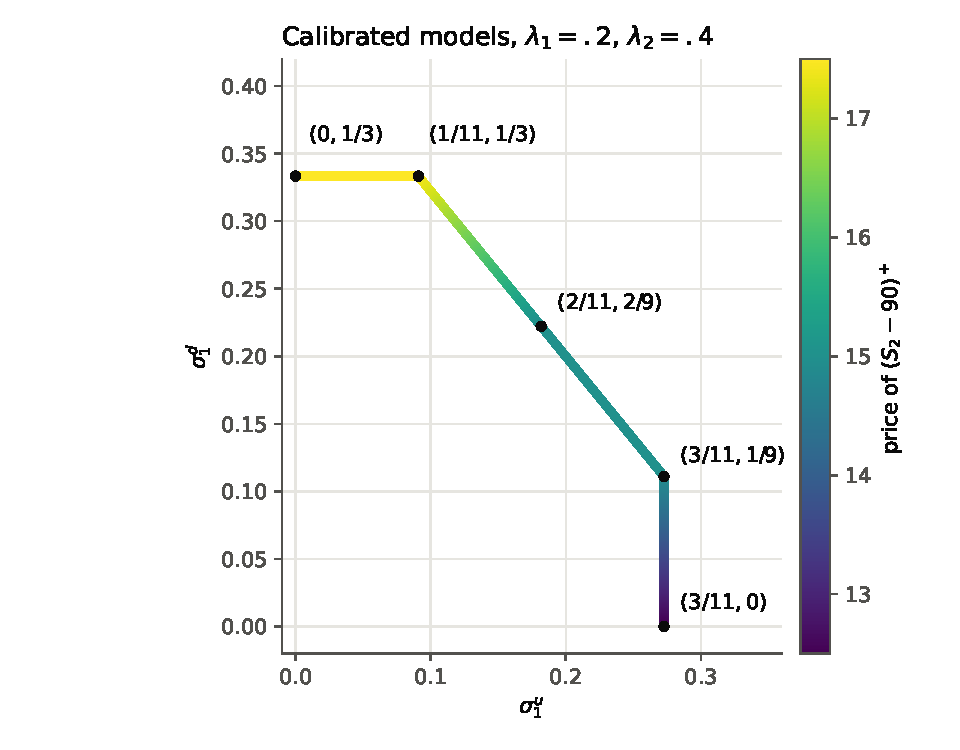
\includegraphics[width=0.78\linewidth]{figures/solution_set.pdf}
\caption{The calibrated set $\mathcal A$, coloured by the price of $(S_2-90)^+$ from Question 5.}
\end{figure}

%-------------------------------------------------------------------------------
\section*{5. Model risk of $X=(S_2-90)^+$, $S_0=100$}
$\sigma_0=.1$, so $S_1^u=110$ and $S_1^d=90$. Leaf by leaf:
\begin{center}\small
\begin{tabular}{lll}\toprule
Leaf & $S_2$ & $(S_2-90)^+$\\\midrule
$uu$ & $110(1+\su)$ & $20+110\su$\\
$ud$ & $110(1-\su)$ & $(20-110\su)^+$, positive iff $\su<2/11$\\
$du$ & $90(1+\sd)$ & $90\sd$\\
$dd$ & $90(1-\sd)$ & $0$\\\bottomrule
\end{tabular}
\end{center}
so
\[
P_a(X)=\tfrac14\bigl[20+110\su+(20-110\su)^++90\sd\bigr].
\]
On each piece of $\mathcal A$:
\begin{itemize}[leftmargin=*]
\item \emph{Horizontal}, $\sd=1/3$, $\su\le1/11<2/11$: $P=\tfrac14[40+30]=17.5$, constant.
\item \emph{Slanted}, $90\sd=40-110\su$. If $\su\le2/11$: $P=\tfrac14[80-110\su]$, falling from $17.5$ to
$15$. If $\su\ge2/11$: the $\su$ terms cancel, $P=\tfrac14[20+40]=15$.
\item \emph{Vertical}, $\su=3/11>2/11$: $P=\tfrac14[50+90\sd]$, from $15$ at $\sd=1/9$ down to $12.5$ at $\sd=0$.
\end{itemize}
$P$ is continuous along $\mathcal A$ and monotone on each piece, so
\begin{align*}
\max_{a\in\mathcal A}P_a(X)&=17.5\quad\bigl(\text{every model with }\sd=\tfrac13,\ \su\le\tfrac1{11}\bigr),\\
\min_{a\in\mathcal A}P_a(X)&=12.5\quad\bigl(\su=\tfrac3{11},\ \sd=0\bigr),
\end{align*}
\[
\boxed{\ \mu_{\mathcal A}(X)=17.5-12.5=5\ }
\]
That is \RangeOverAvg\% of the average model price (\$\AvgArc, averaging along the curve by length; any
average depends on how the models are weighted). The minimum sits at $\sd=0$, a model where the
down node has no volatility. If one insists on $\sigma>0$, $12.5$ is an infimum, not attained, and
$\mu_{\mathcal A}(X)=5$ as a supremum.

\textbf{Why the range is what it is.} Both quoted calls are at the money, and the calibration pins
only what they depend on. At $K=90$ the price picks up the down-up leaf $90\sd$, which the
at-the-money call barely sees, so models that put the time value in the down branch ($\sd=1/3$)
price it high and models that put it in the up branch ($\su=3/11$) price it low. Across strikes:
\begin{center}\small
\begin{tabular}{rrrr}\toprule $K$ & min & max & $\mu_{\mathcal A}$\\\midrule
80 & 20.00 & 25.00 & 5.00\\
90 & 12.50 & 17.50 & 5.00\\
100 & 10.00 & 10.00 & 0.00\\
110 & 2.50 & 7.50 & 5.00\\
120 & 0.00 & 5.00 & 5.00\\
\bottomrule\end{tabular}

\end{center}
At $K=100$ the range is $0$, because that call is a calibration instrument. A range of $0$ there says
nothing about any other strike.

%-------------------------------------------------------------------------------
\section*{Checks}
\begin{itemize}[leftmargin=*]
\item Question 1 and the identity in Question 2 checked by pricing the tree directly at 20{,}000 random
$(\su,\sd)\in[0,1]^2$ (error below $10^{-12}$).
\item Every point of the closed-form $\mathcal A$ reprices $C(2,100)$ to $10$ within $10^{-9}$, and the
smallest $2\max\{\su s_+,\sd s_-\}$ on $\mathcal A$ is $.4>\lambda_1$.
\item A brute-force $1601\times1601$ grid on $[0,1]^2$ finds no calibrated point farther than \GridDist\
from $\mathcal A$, so nothing was missed. The price range of $X$ over those grid points is
\GridLo\ to \GridHi, matching $12.5$ to $17.5$ up to the grid tolerance.
\end{itemize}

\begin{center}
\fbox{\parbox{0.92\textwidth}{\textbf{Carry.}
(1) With $r=0$ and $\pm\sigma$ moves, risk-neutral probabilities are $\tfrac12$; price by listing leaves.
(2) The trick in Q2: decide the sign of each leaf first. $uu$ is always in the money and $dd$ never, so only
the two middle leaves carry a $(\cdot)^+$.
(3) Calibrating 3 parameters to 2 prices leaves a curve of models. Solve it by cases on the kinks.
(4) Model risk is $\max-\min$ of a non-calibrated payoff over that curve. Price it piece by piece; the extremes
sit at the ends of pieces. Exam phrasing: ``which models give the extreme prices, and why?''}}
\end{center}

\appendix
\section{Python source code}
Tree pricing, solution set and checks, \texttt{src/calib.py}:
\lstinputlisting[style=code]{src/calib.py}
Figure and report values, \texttt{src/main.py}:
\lstinputlisting[style=code]{src/main.py}

\end{document}
